% comparison results (number of nodes expanded, time, etc.) for the path finding problemsas the Pacman plans and replans in the environment; figures are helpful here. 


\section{Evaluation}\label{sec:eval}
	\subsection{Metrics}
    The two main metrics used to measure the performance of the three search algorithms were runtime and nodes expanded. Runtime captures the effective amount of time was needed to run the search algorithm and find an optimal path. The runtime was captures by using the linux $\texttt{time}$ command. The other metric nodes expanded, measures the number of nodes that needed to be expanded, i.e. popped from the priority queue in order to complete the search. The nodes expanded metric is linked to both time and space complexity. This is because the more nodes expanded, the longer the search will take. Also, the more nodes expanded, the more space is needed to store those nodes in the queue. Both of these metrics were measured as a function of maze size, i.e. the effective area of a the Pacman maze in test. Note that there is not a direct linear relationship between maze size and search complexity, since the maze size does not capture other factors, such as maze walls. However, the maze size is correlated with search complexity and in general, the larger the maze size, the more complex the search problem.
    
    \subsubsection{Experiments}
    
    \begin{figure}[htb!]
    	\centering
    	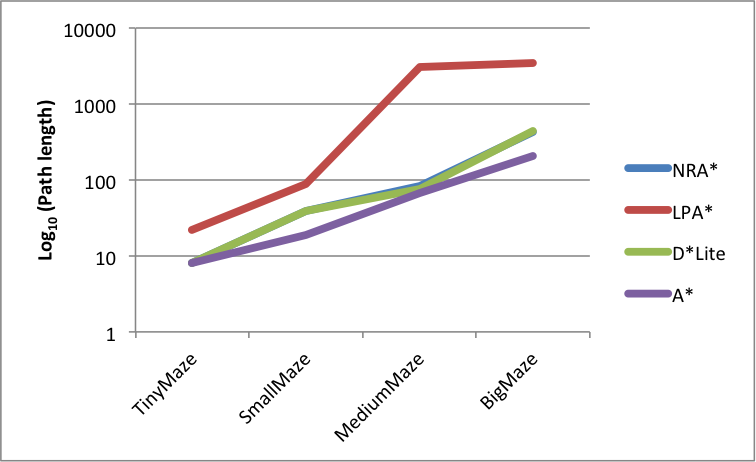
\includegraphics[width=7cm]{PathLength.png}
    	\caption{}
    	\label{fig:1}
    \end{figure}

	\begin{figure}[htb!]
		\centering
		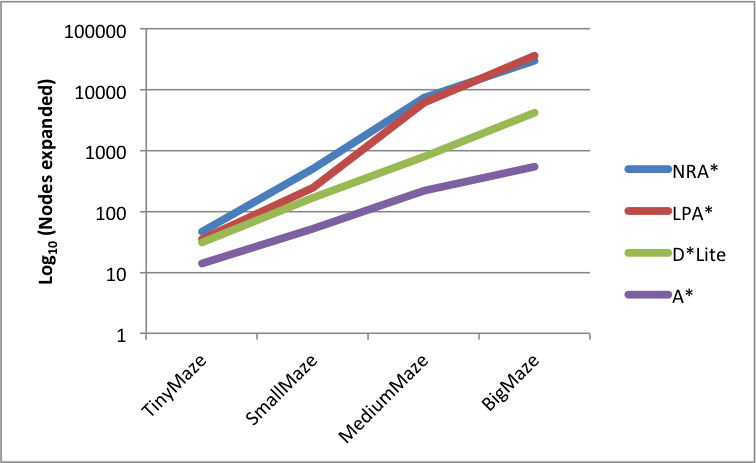
\includegraphics[width=7cm]{NodesExpanded.png}
		\caption{}
		\label{fig:2}
	\end{figure}

	\begin{figure}[htb!]
		\centering
		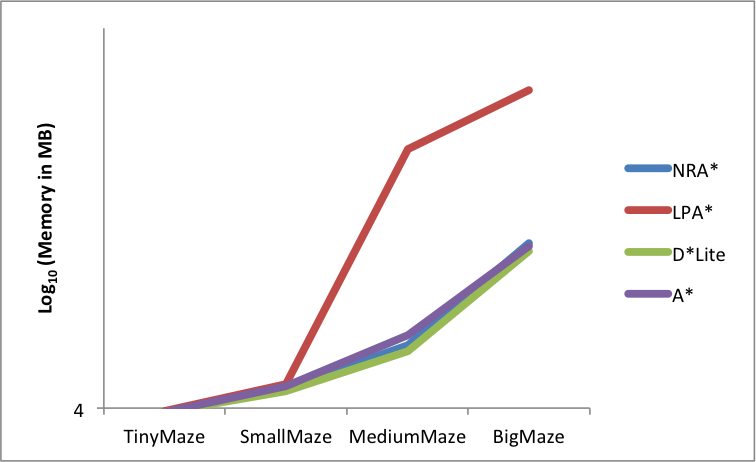
\includegraphics[width=7cm]{Memory.png}
		\caption{}
		\label{fig:3}
	\end{figure}

	\begin{figure}[htb!]
		\centering
		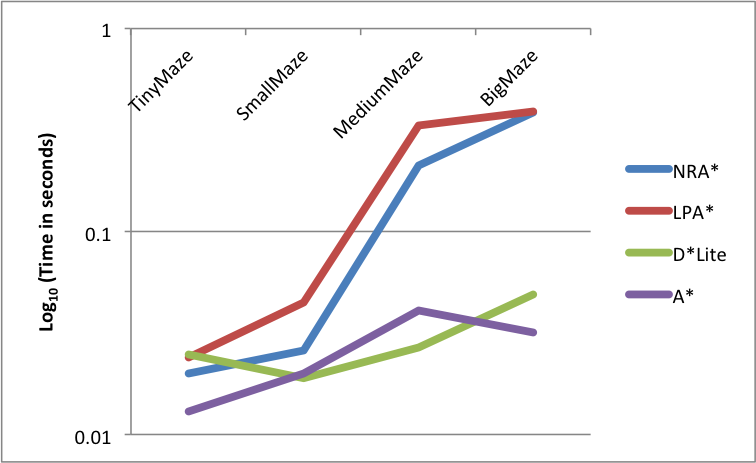
\includegraphics[width=7cm]{Time.png}
		\caption{}
		\label{fig:4}
	\end{figure}

	